\documentclass[letterpaper, 11pt]{article}
\usepackage{comment} % enables the use of multi-line comments (\ifx \fi) 
\usepackage{fullpage} % changes the margin
\usepackage{fancyhdr} % for footerhttps://www.overleaf.com/3039851kkndbp#
\usepackage[UKenglish]{isodate}% http://ctan.org/pkg/isodate for date format
\usepackage{float}%force tables/figs into certain placement
\usepackage{changepage}%for dichotomous key
\usepackage{graphicx}%for figures
\usepackage{subcaption}%for figures
\usepackage{hyperref}%for links
\usepackage[font=small,labelfont=bf]{caption}%for captions
\usepackage[letterpaper,margin=1in]{geometry}
\usepackage{natbib}	%for bibliography
\usepackage{placeins}%prevent images from floating into inappropriate sections

\def\labelitemi{--}

\pagestyle{fancy}
\renewcommand{\headrulewidth}{0pt}

\lhead{}
\chead{}
\rhead{}
\lfoot{ENT 432 (Fall 2015) - Penn State}
\cfoot{}
\rfoot{\thepage}
\renewcommand{\footrulewidth}{0.4pt}
\title{Unit 14 - Antliophora}%check this
\author{}

\begin{document}
\cleanlookdateon %removed ordinal date
\maketitle
\thispagestyle{fancy}
\section*{Introduction}
\textbf{Mecoptera}, \textbf{Siphonaptera}, and \textbf{Diptera} together comprise a lineage called \textbf{Antliophora} (Gr. for ``pump bearers''), insects characterized by the presence of a sperm pump. Diptera is one of the ``big four'' orders of insects, and with \textgreater154,000 described species (15\% of the total estimated diversity) this taxon is a candidate for the most diverse order of insects. 

\section*{Materials}
\begin{itemize}
\item specimens (provided)
\item fine forceps, probes (provided)
\item sorting tray, watch glasses, gloves, safety glasses, glycerine, ethanol (provided)
\item pencil/paper for sketches
\end{itemize}

\section*{Safety}
We will be working with sharp tools and insects on pins. Wear your personal protective gear at all times. Specimens are to be returned to their vials after lab, and glycerine and ethanol will be collected for proper disposal or reuse.

\section*{Methods}
Working with a partner, organize your space, specimens, tools, and microscope. Use your probe and forceps to manipulate the specimen. In this lab, however, we will not be dissecting specimens (unless otherwise noted). You can start anywhere in the handout.

\section{Mecoptera}
Mecoptera and Siphonaptera exhibit some really interesting phenotypes, such as the presence of elongate acanthae in the proventriculus and a unique, resilin-based jumping mechanism. These orders are undoubtedly closely related, with some phylogenies placing Siphonaptera within Mecoptera, sister to Boreidae. This topology, however, is not yet a robust estimation of relationships, and we treat them separately in lab. Mecoptera exhibit the following characters:
\begin{itemize}
\item fore wing (if present) with \textless4 costal crossveins, 20+ closed cells
\item head prolonged below eyes as a beak or rostrum, with chewing mouthparts at tip
\end{itemize}

\subsection{Panorpidae (scorpionflies)}
\begin{itemize}
\item tarsi not raptorial, and with two small claws apically
\item wings fairly broad at base
\item male genitalia somewhat resemble scorpion sting
\end{itemize}

\begin{figure}[ht!]
  \centering
    
\includegraphics[width=0.3\textwidth]{blank}
  \caption{Panorpidae}
  \label{fig:panorpid}
\end{figure}

\subsection{Bittacidae (hangingflies)}
\begin{itemize}
\item tarsi each with one large claw
\item tarsi raptorial, tarsomere 5 fold back against tarsomere 4
\item wings narrower at base
\item usually crane fly like in appearance, occasionally wingless
\end{itemize}
Compare the leg morphology of these insects to Panorpidae. Can you predict how the legs function? What adaptations do you see?\vspace{3cm}

\begin{figure}[ht!]
    \centering
    \begin{subfigure}[ht!]{0.25\textwidth}
        
\includegraphics[width=\textwidth]{blank}
        \caption{}
        \label{fig:bittac1}
    \end{subfigure}
    \qquad %add desired spacing between images, e. g. ~, \quad, \qquad, \hfill etc. 
      %(or a blank line to force the subfigure onto a new line)
    \begin{subfigure}[ht!]{0.5\textwidth}
        
\includegraphics[width=\textwidth]{blank}
        \caption{}
        \label{fig:bittac2}
    \end{subfigure}
    \caption{Bittacidae}\label{fig:bittacids}
\end{figure}

\subsection{Boreidae (snow scorpionflies)}
\begin{itemize}
\item body usually mostly brown or black 
\item antennae long
\item wings vestigial and hind legs long, saltatorial (may not be obvious unless you examine internal characters)
\item female has a straight ovipositor about the same length as the rostrum
\item males have a blunt, rounded abdominal tip
\end{itemize}

\begin{figure}[ht!]
  \centering
    
\includegraphics[width=0.5\textwidth]{blank}
  \caption{Boreidae}
  \label{fig:boreid}
\end{figure}

\section{Siphonaptera (fleas)}
\begin{itemize}
\item usually small, laterally flattened ectoparasites of vertebrates
\item wingless, laterally flattened, spiny
\item antennae small, set back in grooves (scrobes) on the head
\item eyes reduced in size
\item legs adapted in part for jumping
\end{itemize}
Given the above characters and others you observe on the specimens we have in lab, describe three adaptations to living and feeding on a mammalian host.\vspace{3cm}

\subsection{Pulicidae (dog, cat fleas)}
\begin{itemize}
\item mid coxa without internal ridge
\item hind tibia without apical tooth
\end{itemize}

\begin{figure}[ht!]
  \centering
    
\includegraphics[width=0.6\textwidth]{blank}
  \caption{Pulicidae}
  \label{fig:pulicid}
\end{figure}

\section{Diptera (true flies)}
\begin{itemize}
\item palps with 1--5 segments
\item 1--5 branches of R (Figure \ref{fig:dipteranwing})
\item hind wing (haltere) relatively small, knob-like
\end{itemize}

\begin{figure}[ht!]
  \centering
    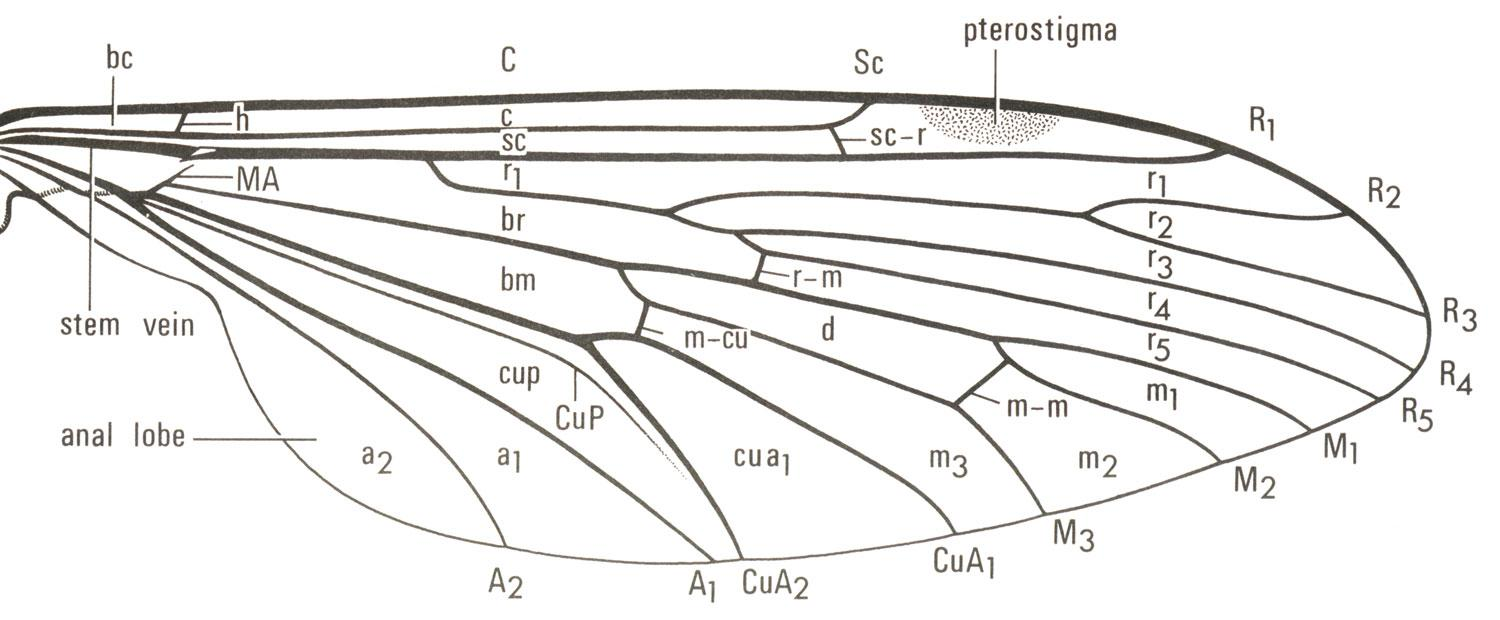
\includegraphics[width=0.75\textwidth]{DipteraWing}
  \caption{Diptera, generalized fore wing \citep[][Fig. 67]{mcalpine1981manual}}
  \label{fig:dipteranwing}
\end{figure}

\subsection{Non-Brachycera (``Nematocera'')}
\begin{itemize}
\item fragile, often with long legs 
\item antenna with 4+ freely articulated flagellomeres
\end{itemize}
This paraphyletic (hence the quotes around the name) group of taxa is comprised of species that have retained a lot of ancestral characters. 

\subsubsection{Tipulidae (crane flies)}
\noindent{}\textit{Diagnostic characters:} Ocelli absent; antennae slender but relatively short; mesonotum with V-shaped suture; wing with many veins; 2 anal veins reach margin; legs relatively long, autotomic (easily shed)\\

\noindent{}\textit{Natural history:} \\

\noindent\textbf{Question 1:} In what other taxa have we seen autotomic appendages, and why is it relevant?\\

\begin{figure}[ht!]
    \centering
    \begin{subfigure}[ht!]{0.4\textwidth}
        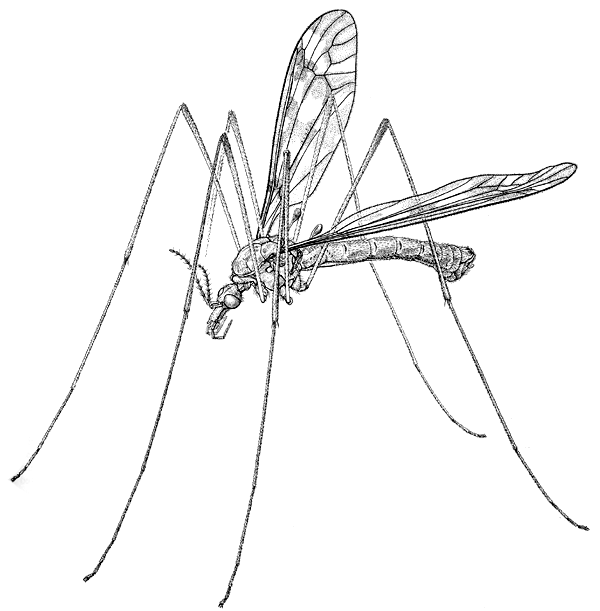
\includegraphics[width=\textwidth]{TipulidHabitus}
        \caption{Habitus \citep[][Fig. 7.1]{mcalpine1981manual}}
        \label{fig:tipulid1}
    \end{subfigure}
    \qquad 
    \begin{subfigure}[ht!]{0.45\textwidth}
        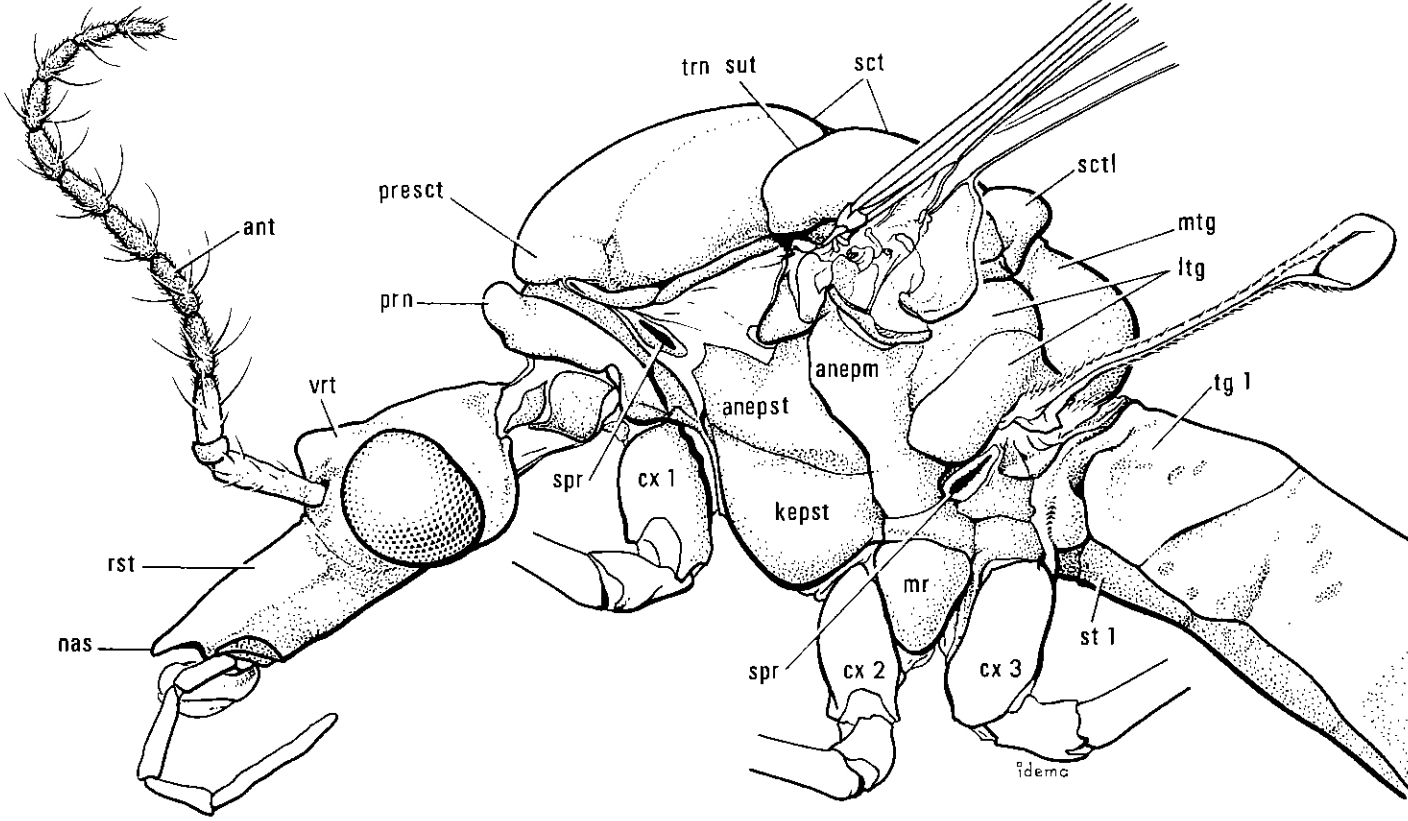
\includegraphics[width=\textwidth]{TipulidThorax}
        \caption{Lateral thorax and head \citep[][Fig. 7.2]{mcalpine1981manual}}
        \label{fig:tipulid2}
    \end{subfigure}
    \caption{Tipulidae}\label{fig:tipulids}
\end{figure}

\subsubsection{Simuliidae (black flies)}
\noindent{}\textit{Diagnostic characters:} Stout-bodied, humpbacked, \textless3 mm; ocelli absent; antennae as long as or shorter than head (but still filiform); wings broad, anterior veins thick, posterior veins weakly sclerotized.\\

\noindent{}\textit{Natural history:} \\

\begin{figure}[ht!]
    \centering
    \begin{subfigure}[ht!]{0.32\textwidth}
        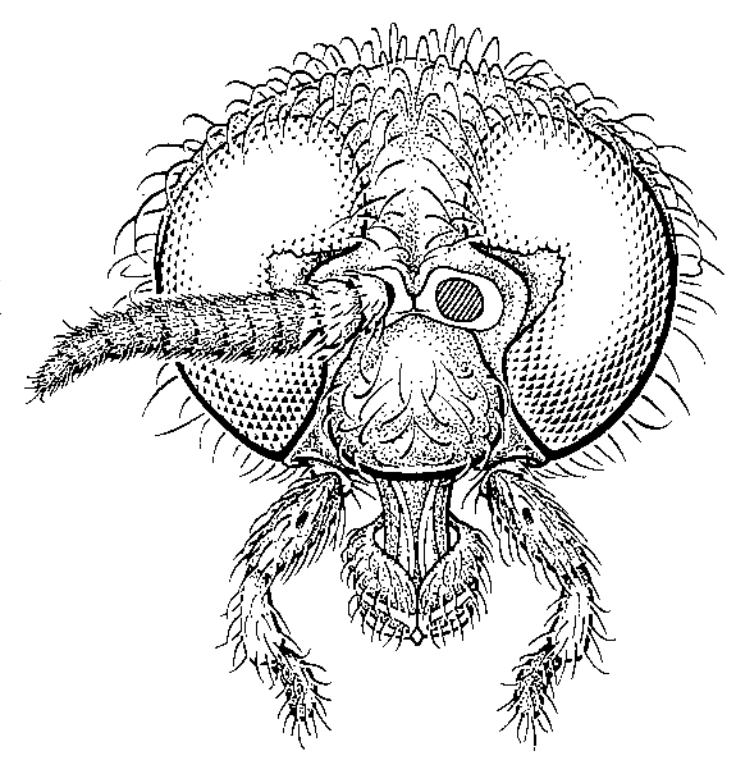
\includegraphics[width=\textwidth]{SimuliidHead}
        \caption{Head \citep[][Fig. 27.5]{mcalpine1981manual}}
        \label{fig:simuliid1}
    \end{subfigure}
    \qquad 
    \begin{subfigure}[ht!]{0.42\textwidth}
        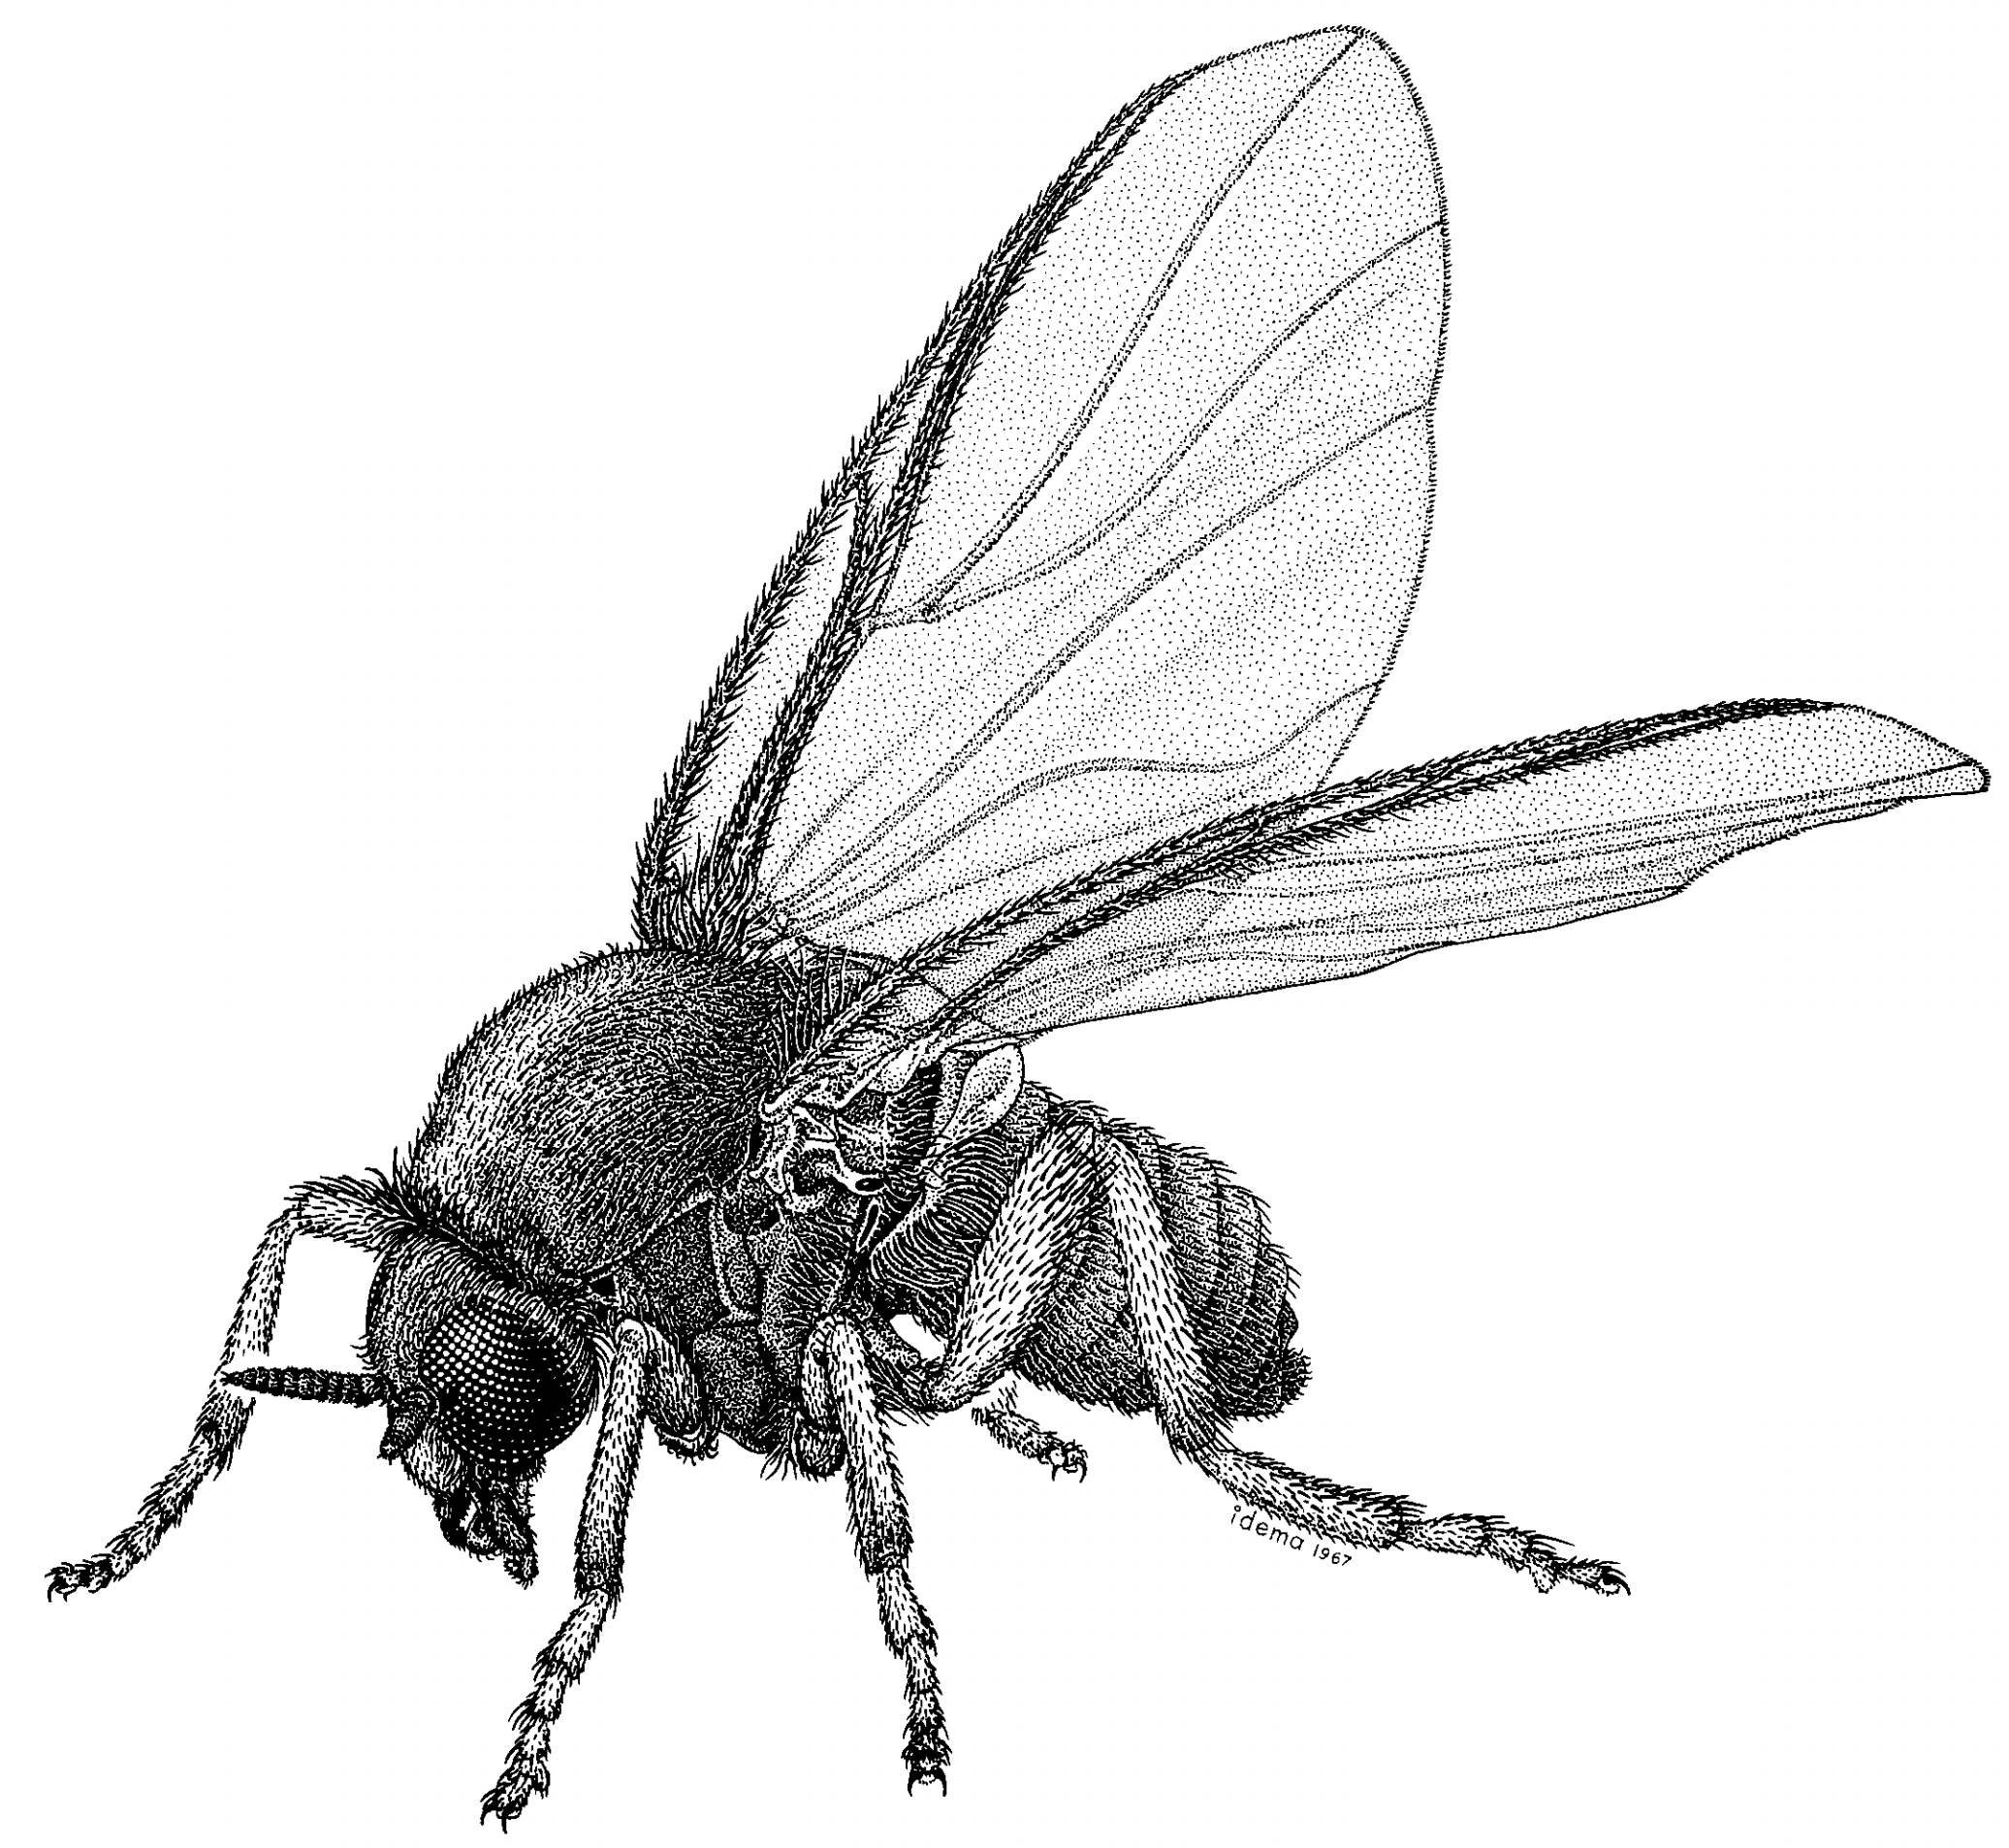
\includegraphics[width=\textwidth]{SimuliidHabitus}
        \caption{Lateral thorax and head \citep[][Fig. 27.1]{mcalpine1981manual}}
        \label{fig:simuliid2}
    \end{subfigure}
    \caption{Simuliidae}\label{fig:simuliids}
\end{figure}

\subsubsection{Chironomidae (midges)}
\noindent{}\textit{Diagnostic characters:} Ocelli absent; antennae usually plumose, more so in males; mouthparts without mandibles; legs long, fore leg longer than others; fore wing M unbranched.\\

\noindent{}\textit{Natural history:} \\

\begin{figure}[ht!]
    \centering
    \begin{subfigure}[ht!]{0.45\textwidth}
        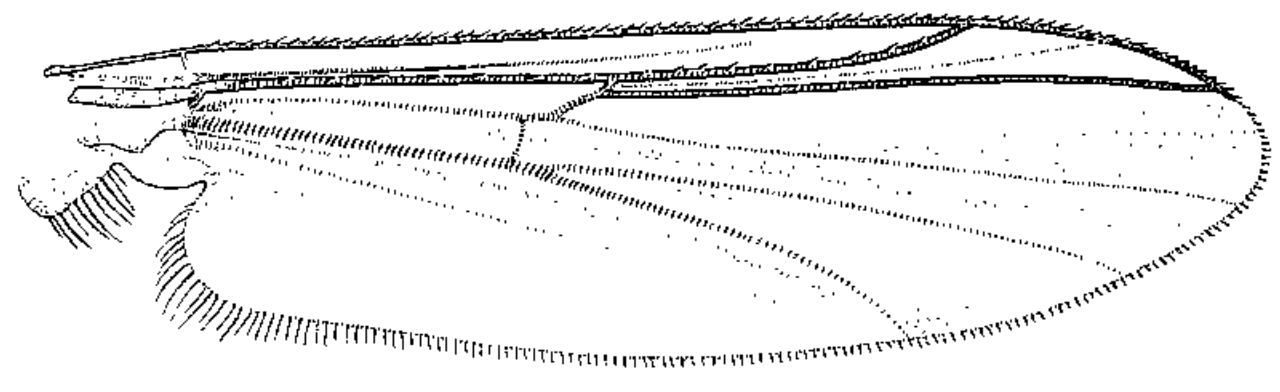
\includegraphics[width=\textwidth]{ChironomidWing}
        \caption{Fore wing \citep[][Fig. 29.9]{mcalpine1981manual}}
        \label{fig:chiron1}
    \end{subfigure}
    \qquad 
    \begin{subfigure}[ht!]{0.45\textwidth}
        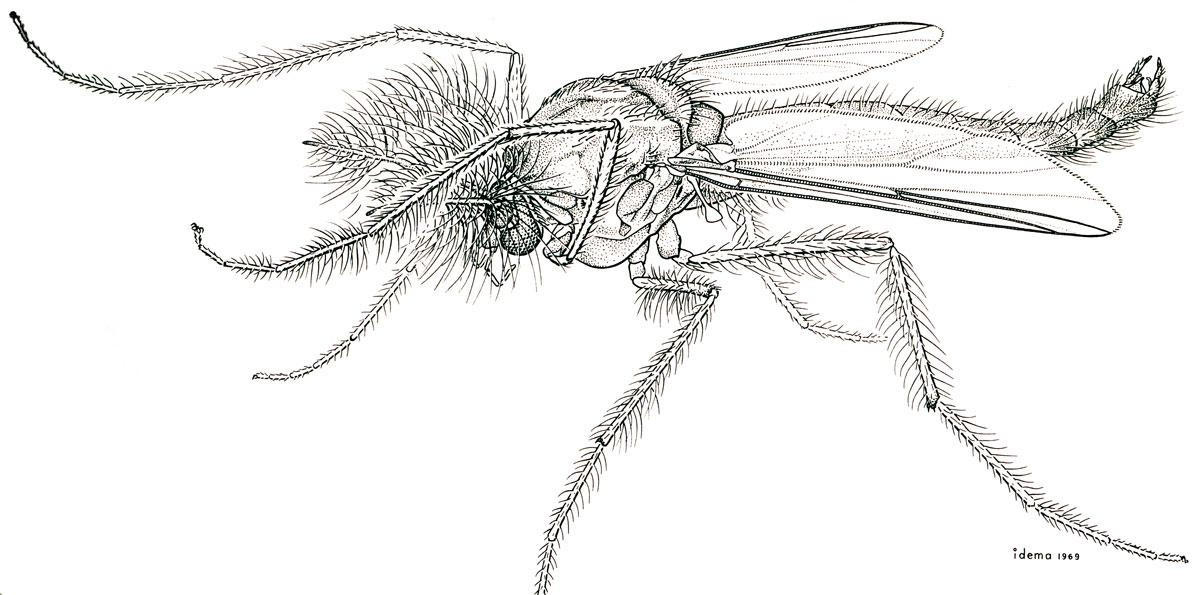
\includegraphics[width=\textwidth]{ChironomidHabitus}
        \caption{Habitus \citep[][Fig. 29.1]{mcalpine1981manual}}
        \label{fig:chiron2}
    \end{subfigure}
    \caption{Chironomidae}\label{fig:chironomids}
\end{figure}

\subsubsection{Ceratopogonidae (biting midges, no-see-ums, punkies)}
\noindent{}\textit{Diagnostic characters:} Mouthparts with mandibles; fore wing M branched into 2--3 veins; legs relatively short. \\%needs more! small stature, eyes?

\noindent{}\textit{Natural history:} \\

\begin{figure}[ht!]
    \centering
    \begin{subfigure}[ht!]{0.3\textwidth}
        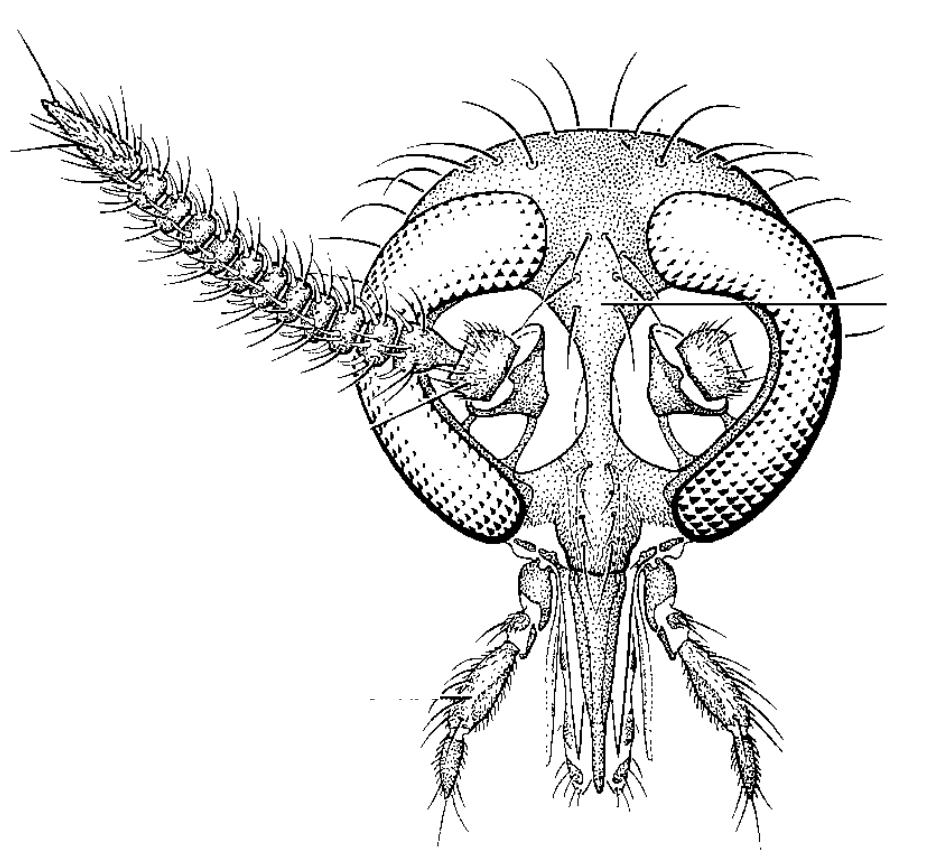
\includegraphics[width=\textwidth]{CeratopogonidHead}
        \caption{Head in anterior view \citep[][Fig. 28.4]{mcalpine1981manual}}
        \label{fig:ceratopogonid1}
    \end{subfigure}
    \qquad 
    \begin{subfigure}[ht!]{0.45\textwidth}
        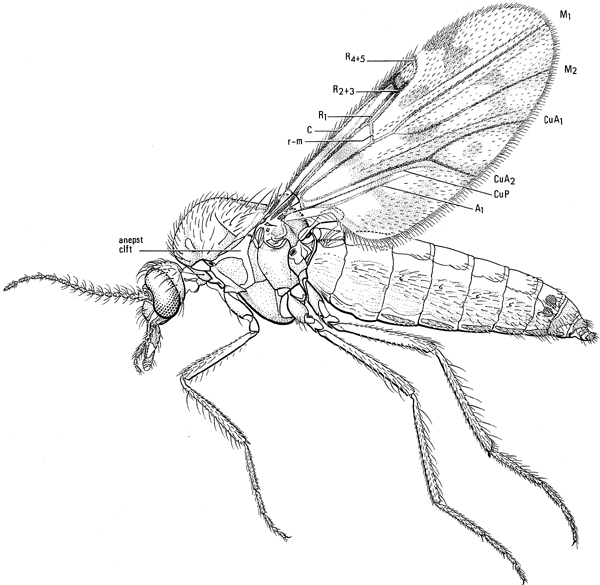
\includegraphics[width=\textwidth]{CeratopogonidHabitus}
        \caption{Habitus \citep[][Fig. 28.13]{mcalpine1981manual}}
        \label{fig:ceratopogonid2}
    \end{subfigure}
    \caption{Ceratopogonidae}\label{fig:ceratopogonids}
\end{figure}

\subsubsection{Culicidae (mosquitoes)}
\noindent{}\textit{Diagnostic characters:} Body, especially wings often scaly; ocelli absent; proboscis long; antennae plumose, more so in males; wings narrow, with scales on veins.\\

\noindent{}\textit{Natural history:} \\

\begin{figure}[ht!]
    \centering
    \begin{subfigure}[ht!]{0.45\textwidth}
        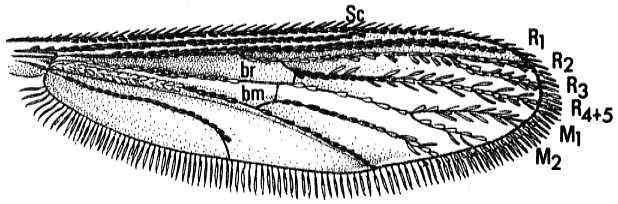
\includegraphics[width=\textwidth]{CulicidWing}
        \caption{Fore wing, with scales \citep[][Fig. 25.5]{mcalpine1981manual}}
        \label{fig:culic1}
    \end{subfigure}
    \qquad
    \begin{subfigure}[ht!]{0.45\textwidth}
        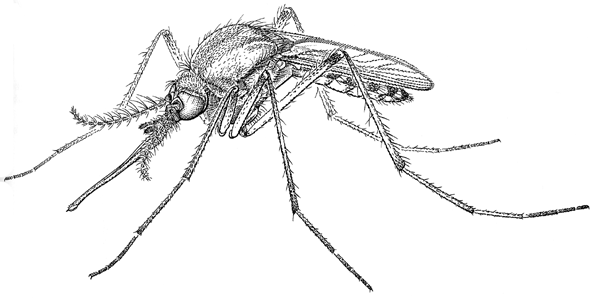
\includegraphics[width=\textwidth]{CulicidHabitus}
        \caption{Habitus \citep[][Fig. 25.1]{mcalpine1981manual}}
        \label{fig:culic2}
    \end{subfigure}
    \caption{Culicidae}\label{fig:culicids}
\end{figure}

\subsubsection{Psychodidae (moth, sand, drain flies)}
\noindent{}\textit{Diagnostic characters:} Small to minute, stout and very setose;  antennae with characteristic setae rings; ocelli absent; wings broad oval, tapering apically, hairy, venation distinct; fore wing R 4-branched, with straight veins, few crossveins, and transverse fold near base of wing.\\

\noindent{}\textit{Natural history:} \\

\begin{figure}[ht!]
    \centering
    \begin{subfigure}[ht!]{0.4\textwidth}
        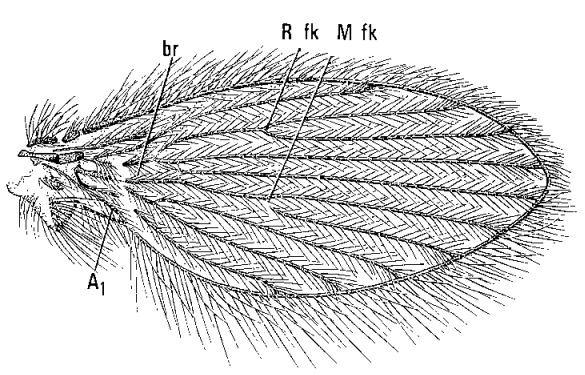
\includegraphics[width=\textwidth]{PsychodidWing}
        \caption{Fore wing, with scales \citep[][Fig. 17.11]{mcalpine1981manual}}
        \label{fig:psychodid1}
    \end{subfigure}
    \qquad
    \begin{subfigure}[ht!]{0.45\textwidth}
        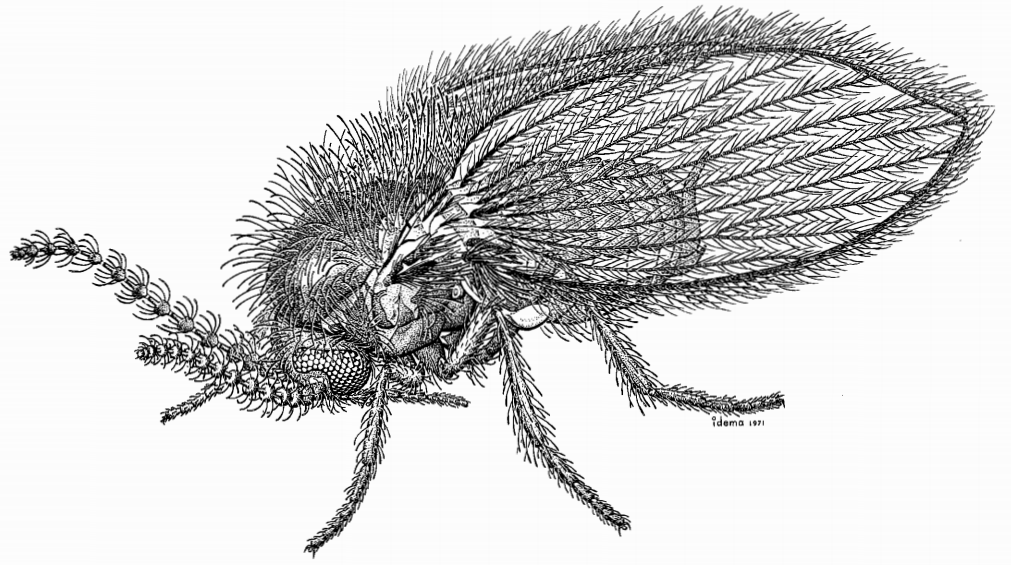
\includegraphics[width=\textwidth]{PsychodidHabitus}
        \caption{Habitus \citep[][Fig. 17.1]{mcalpine1981manual}}
        \label{fig:psychodid2}
    \end{subfigure}
    \caption{Psychodidae}\label{fig:psychodids}
\end{figure}

\subsubsection{Cecidomyiidae (gall midges)}
\noindent{}\textit{Diagnostic characters:} Eyes usually meet above antennae; wing venation reduced, \textless7 prominent veins reach margin; C continues around wing apex, though weaker posteriorly; first tarsal segment very small; antennae and legs long, slender.\\%can't we do better?

\noindent{}\textit{Natural history:} \\

\begin{figure}[ht!]
    \centering
    \begin{subfigure}[ht!]{0.45\textwidth}
        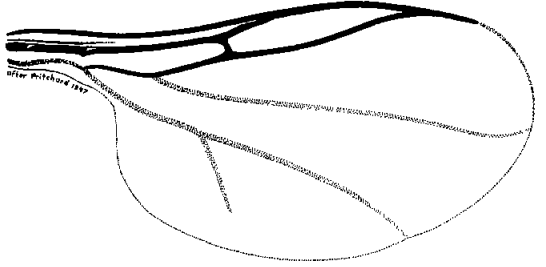
\includegraphics[width=\textwidth]{CecidomyiidWing}
        \caption{Fore wing \citep[][Fig. 16.13]{mcalpine1981manual}}
        \label{fig:cecidomyiid1}
    \end{subfigure}
    \qquad
    \begin{subfigure}[ht!]{0.25\textwidth}
        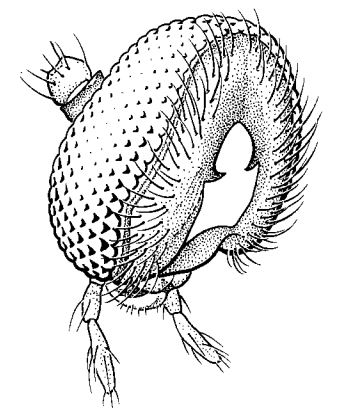
\includegraphics[width=\textwidth]{CecidomyiidHead}
        \caption{Habitus \citep[][Fig. 16.2]{mcalpine1981manual}}
        \label{fig:cecidomyiid2}
    \end{subfigure}
    \caption{Cecidomyiidae}\label{fig:cecidomyiids}
\end{figure}

\subsubsection{Sciaridae (dark-winged fungus gnats)}
\noindent{}\textit{Diagnostic characters:} Usually mostly black or dark brown in color; eyes meet above antennae; ocelli present; wing venation reduced, usually \textless7 prominent veins reach margin; C ends at wing tip.\\

\noindent{}\textit{Natural history:} \\

\begin{figure}[ht!]
    \centering
    \begin{subfigure}[ht!]{0.45\textwidth}
        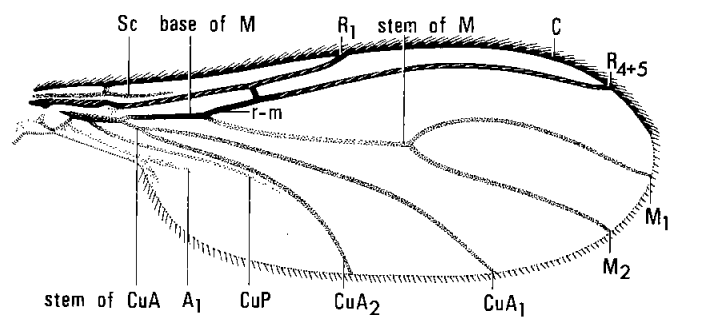
\includegraphics[width=\textwidth]{SciaridWing}
        \caption{Fore wing \citep[][Fig. 15.19]{mcalpine1981manual}}
        \label{fig:sciarid1}
    \end{subfigure}
    \qquad
    \begin{subfigure}[ht!]{0.25\textwidth}
        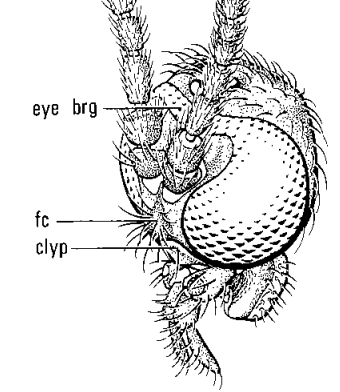
\includegraphics[width=\textwidth]{SciaridHead}
        \caption{Habitus \citep[][Fig. 15.4]{mcalpine1981manual}}
        \label{fig:sciarid2}
    \end{subfigure}
    \caption{Sciaridae}\label{fig:sciarids}
\end{figure}

\subsubsection{Bibionidae (March flies)}
\noindent{}\textit{Diagnostic characters:} Body with many erect bristles (\textit{i.e.}, ``hairy''), usually black; male head shape different from female; ocelli present; antennae shorter than thorax, arising low on face; basal M cell present; anal angle of wing somewhat enlarged.\\

\noindent{}\textit{Natural history:} \\

\begin{figure}[ht!]
    \centering
    \begin{subfigure}[ht!]{0.25\textwidth}
        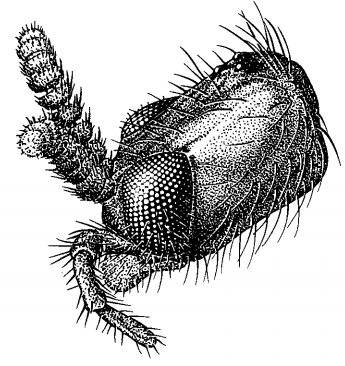
\includegraphics[width=\textwidth]{BibionidHead}
        \caption{Female head in lateral view \citep[][Fig. 13.3]{mcalpine1981manual}}
        \label{fig:bibionid1}
    \end{subfigure}
    \qquad
    \begin{subfigure}[ht!]{0.47\textwidth}
        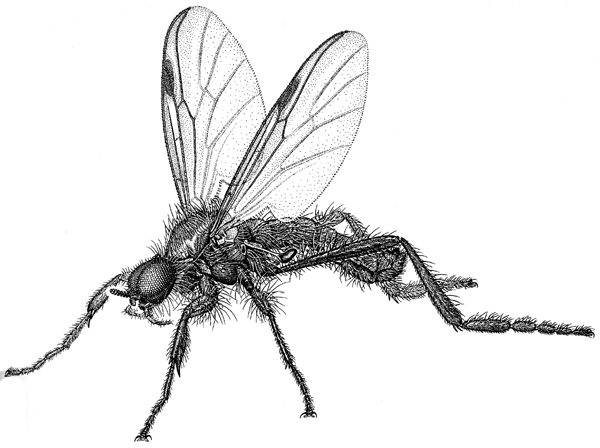
\includegraphics[width=\textwidth]{BibionidHabitus}
        \caption{Male habitus \citep[][Fig. 13.1]{mcalpine1981manual}}
        \label{fig:bibionid2}
    \end{subfigure}
    \caption{Bibionidae}\label{fig:bibionids}
\end{figure}

\subsubsection{Mycetophilidae (fungus gnats)}
\noindent{}\textit{Diagnostic characters:} Head often concealed in dorsal view; ocelli present; antennae longer than thorax; eyes do not meet above antennae; coxae relatively elongate.\\

\noindent{}\textit{Natural history:} \\

\begin{figure}[ht!]
    \centering
    \begin{subfigure}[ht!]{0.45\textwidth}
        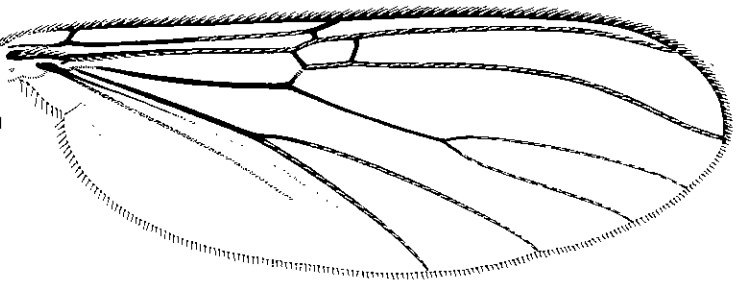
\includegraphics[width=\textwidth]{MycetophilidWing}
        \caption{Fore wing \citep[][Fig. 14.24]{mcalpine1981manual}}
        \label{fig:mycetophilid1}
    \end{subfigure}
    \qquad
    \begin{subfigure}[ht!]{0.27\textwidth}
        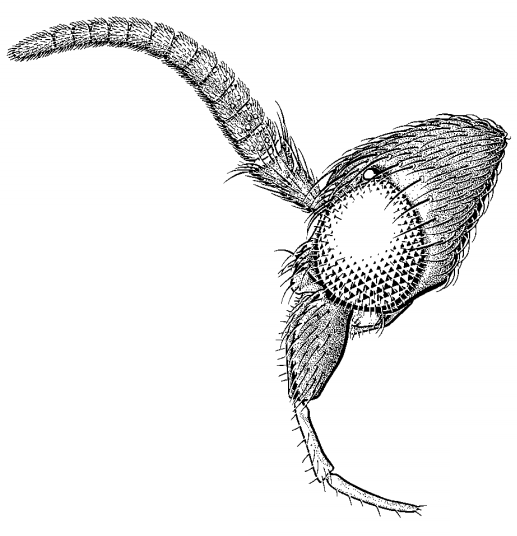
\includegraphics[width=\textwidth]{MycetophilidHead}
        \caption{Head in lateral view \citep[][Fig. 13.1]{mcalpine1981manual}}
        \label{fig:mycetophilid2}
    \end{subfigure}
    \caption{Mycetophilidae}\label{fig:mycetophilids}
\end{figure}

\subsection{Brachycera (short-horned flies)}
\begin{itemize}
\item generally stouter bodied than ``Nematocera''
\item flagellum at least partly fused, with \textless5 articulations, very rarely \textgreater10
\item palps with 0--2 segments
\end{itemize}
Unlike ``Nematocera'', this suborder is demonstrably monophyletic. There have been several attempts to subdivide this taxon, but each scheme usually results in one paraphyletic group and one monophyletic group.

\subsubsection{Stratiomyidae (soldier flies)}
\noindent{}\textit{Diagnostic characters:} Often mimics of wasps or bees; 3rd antennal segment elongate, annulate or rounded, with arista; fore wing d cell round, not elongate, Rs bunched near anterior margin, R4 and R5 fork anterior to wing tip, C ends before wing tip.\\

\noindent{}\textit{Natural history:} \\

\begin{figure}[ht!]
    \centering
    \begin{subfigure}[ht!]{0.5\textwidth}
        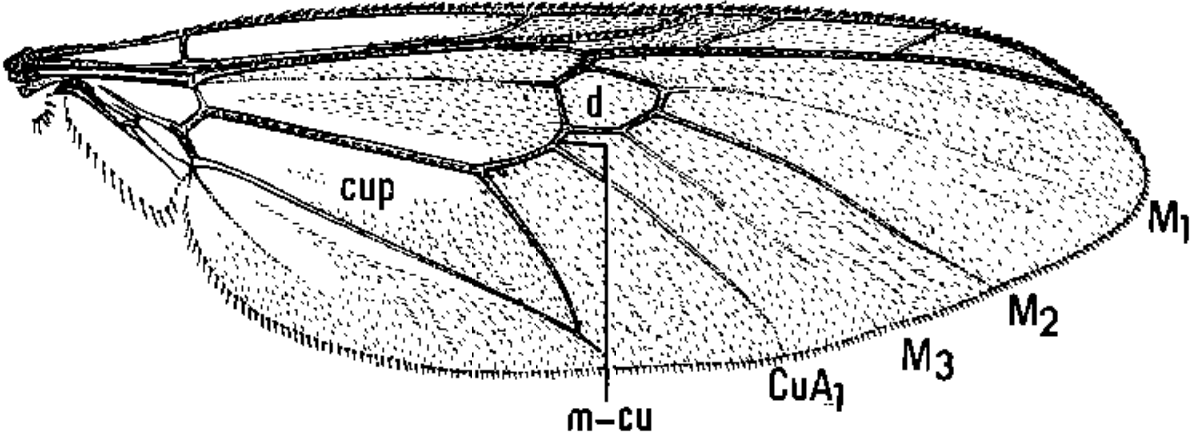
\includegraphics[width=\textwidth]{StratiomyidWing}
        \caption{Fore wing \citep[][Fig. 36.33]{mcalpine1981manual}}
        \label{fig:stratiomyid1}
    \end{subfigure}
    \qquad
    \begin{subfigure}[ht!]{0.2\textwidth}
        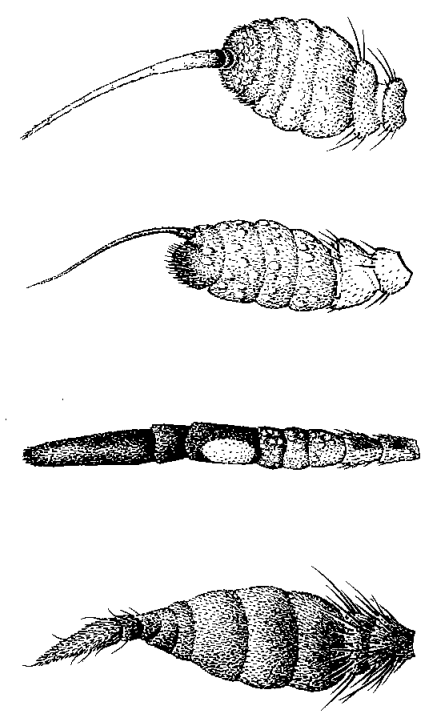
\includegraphics[width=\textwidth]{StratiomyidAntennae}
        \caption{Antenna variation \citep[][Figs. 36.9,12,15,18]{mcalpine1981manual}}
        \label{fig:stratiomyid2}
    \end{subfigure}
    \caption{Stratiomyidae}\label{fig:stratiomyids}
\end{figure}

\subsubsection{Tabanidae (horse and deer flies)}
\noindent{}\textit{Diagnostic characters:} Mouthparts modified for sucking blood and nectar; eyes often with iridescent patterns; 3rd antennal segment never aristate; fore wing R4 and R5 fork encloses wing tip, d cell elongate; postscutellum present; first visible abdominal tergite divided dorsally.\\

\noindent{}\textit{Natural history:} \\

\begin{figure}[ht!]
    \centering
    \begin{subfigure}[ht!]{0.4\textwidth}
        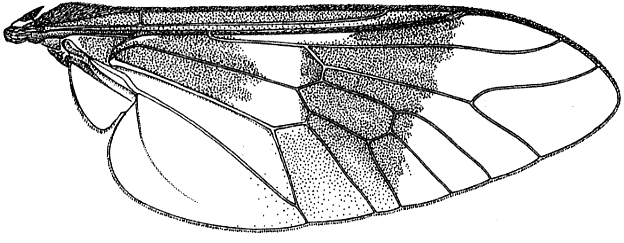
\includegraphics[width=\textwidth]{TabanidWing}
        \caption{Fore wing \citep[][Fig. 31.35]{mcalpine1981manual}}
        \label{fig:tabanid1}
    \end{subfigure}
    \qquad
    \begin{subfigure}[ht!]{0.5\textwidth}
        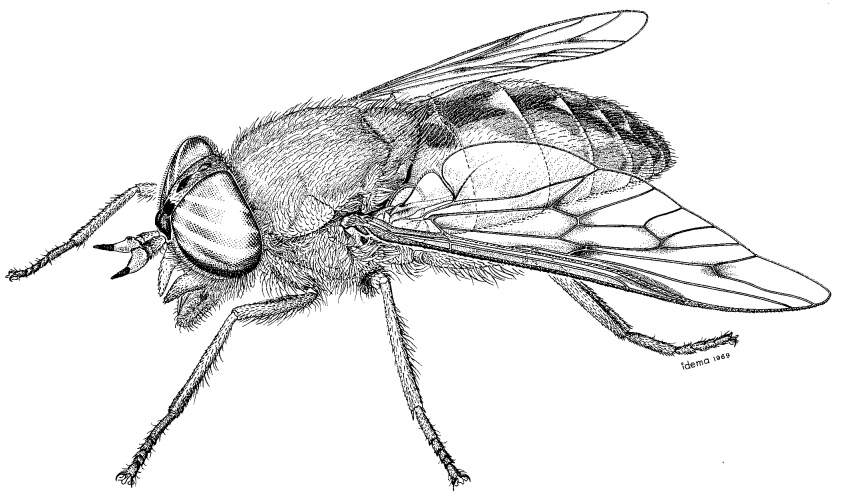
\includegraphics[width=\textwidth]{TabanidHabitus}
        \caption{Habitus \citep[][Fig. 31.1]{mcalpine1981manual}}
        \label{fig:tabanid2}
    \end{subfigure}
    \caption{Tabanidae}\label{fig:tabanids}
\end{figure}

\subsubsection{Asilidae (robber flies)}
\noindent{}\textit{Diagnostic characters:} Medium-sized to large flies, variable but often mimicking bees or with elongate, tapering abdomen; top of head (vertex) distinctly depressed between eyes; face with mystax (mustache); mouthparts heavily sclerotized, pointed, for piercing; fore wing CuA2 reaches wing margin or joins A1 near margin.\\

\noindent{}\textit{Natural history:} \\

\begin{figure}[ht!]
    \centering
    \begin{subfigure}[ht!]{0.25\textwidth}
        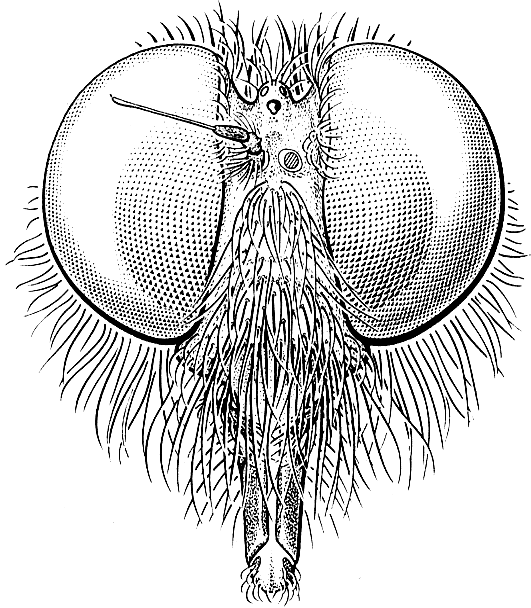
\includegraphics[width=\textwidth]{AsilidHead}
        \caption{Head \citep[][Fig. 42.35]{mcalpine1981manual}}
        \label{fig:asilid2}
    \end{subfigure}
    \qquad 
    \begin{subfigure}[ht!]{0.45\textwidth}
        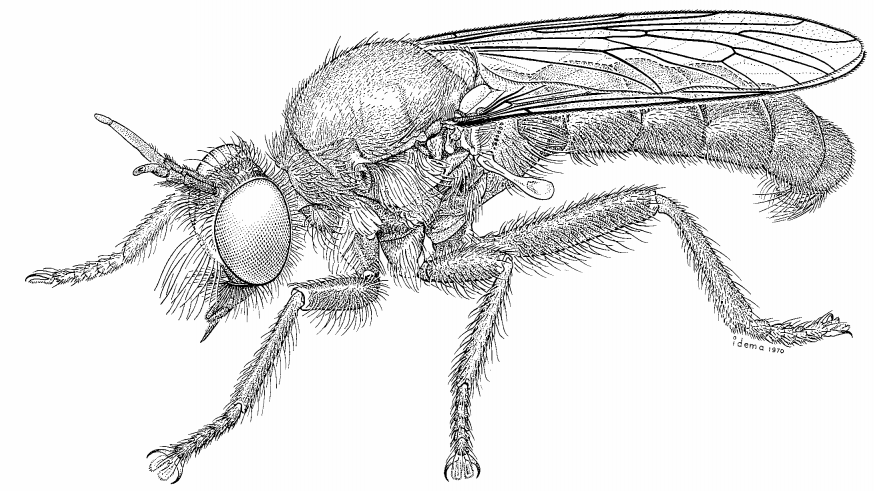
\includegraphics[width=\textwidth]{AsilidHabitus}
        \caption{Habitus \citep[][Fig. 42.1]{mcalpine1981manual}}
        \label{fig:asilid1}
    \end{subfigure}
    \caption{Asilidae}\label{fig:asilids}
\end{figure}

\subsubsection{Bombyliidae (bee flies)}
\noindent{}\textit{Diagnostic characters:} Extremely variable in form and size but commonly hairy and stout, mimicking bees; proboscis often slender and long;; wing venation variable but veins often strongly curved anteriorly; CuA2 reaches wing margin or joins A1 near margin; cell bm with 3 corners on the end.\\

\noindent{}\textit{Natural history:} \\

\begin{figure}[ht!]
    \centering
    \begin{subfigure}[ht!]{0.45\textwidth}
        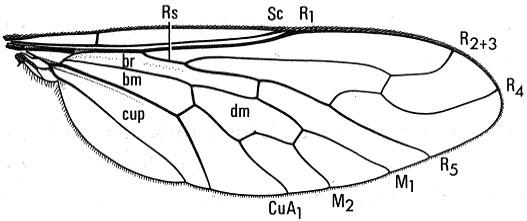
\includegraphics[width=\textwidth]{BombyliidWing}
        \caption{Fore wing \citep[][Fig. 45.1]{mcalpine1981manual}}
        \label{fig:bombyl2}
    \end{subfigure}
    \qquad 
    \begin{subfigure}[ht!]{0.4\textwidth}
        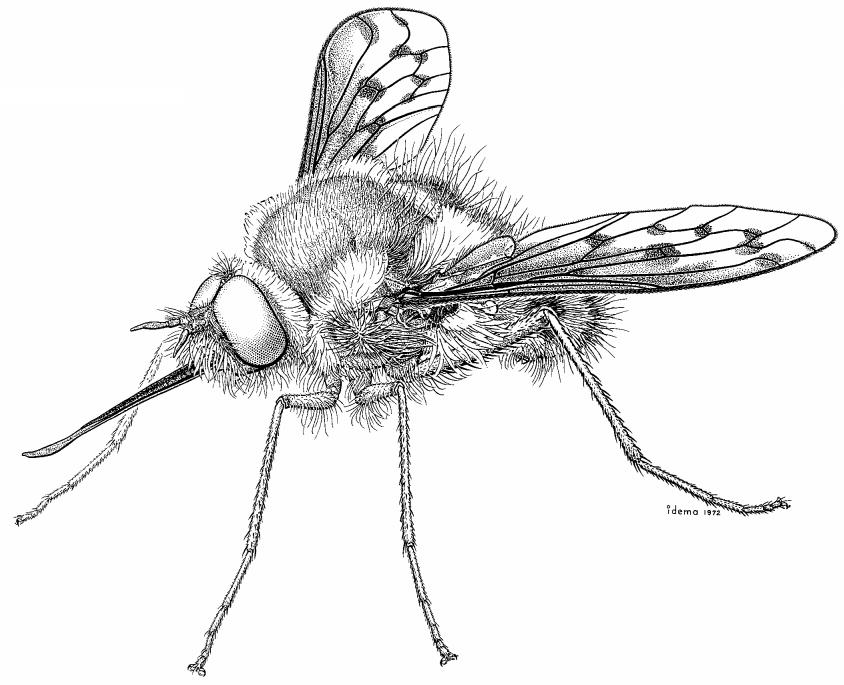
\includegraphics[width=\textwidth]{BombyliidHabitus}
        \caption{Habitus \citep[][Fig. 45.1]{mcalpine1981manual}}
        \label{fig:bombyl1}
    \end{subfigure}
    \caption{Bombyliidae}\label{fig:bombyls}
\end{figure}

\paragraph{Eremoneura} The remaining flies belong to Eremoneura.

\subsubsection{Dolichopodidae (long-legged flies)}
\noindent{}\textit{Diagnostic characters:} Long-legged and usually metallic green or coppery; head shape is distinctive; antennae usually aristate; CuA2 joins A1 far from margin; Rs 2-branched, branches, r-m crossvein crowded near wing base, anal cell small or absent; male genitalia often large and folded under abdomen.

\noindent{}\textit{Natural history:} \\

\begin{figure}[ht!]
    \centering
    \begin{subfigure}[ht!]{0.5\textwidth}
        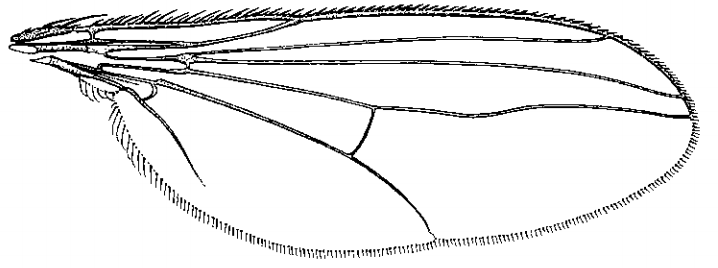
\includegraphics[width=\textwidth]{DolichopodidWing}
        \caption{Fore wing \citep[][Fig. 48.30]{mcalpine1981manual}}
        \label{fig:dolicho1}
    \end{subfigure}
    \qquad
    \begin{subfigure}[ht!]{0.22\textwidth}
        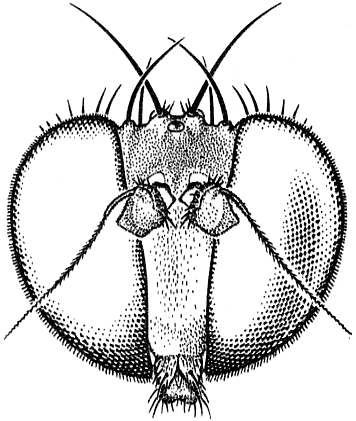
\includegraphics[width=\textwidth]{DolichopodidHead}
        \caption{Head \citep[][Fig. 48.4]{mcalpine1981manual}}
        \label{fig:dolicho2}
    \end{subfigure}
    \caption{Dolichopodidae}\label{fig:dolichos}
\end{figure}

\subsubsection{Empididae (dance flies)}
\noindent{}\textit{Diagnostic characters:} Body variable in shape but usually hump-backed, dome-shaped, and colorful but not metallic; 3rd antennal stylate or aristate; CuA2 joins A1 far from margin (look for large open cell in lower part of wing); wing venation otherwise variable, R 2--3-branched, branches and r-m crossvein arise distally.\\ %check venation

\noindent{}\textit{Natural history:} \\

\begin{figure}[ht!]
    \centering
    \begin{subfigure}[ht!]{0.45\textwidth}
        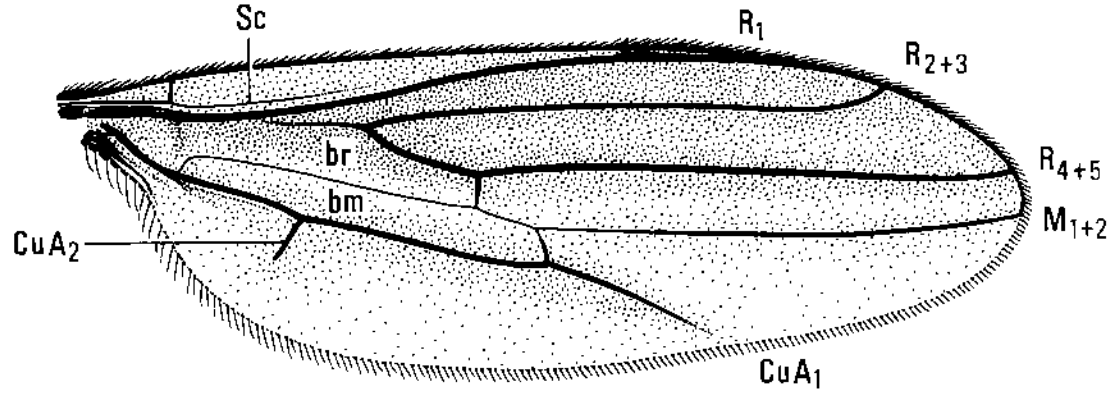
\includegraphics[width=\textwidth]{EmpididWing}
        \caption{Fore wing \citep[][Fig. 47.3]{mcalpine1981manual}}
        \label{fig:empidid1}
    \end{subfigure}
    \qquad
    \begin{subfigure}[ht!]{0.42\textwidth}
        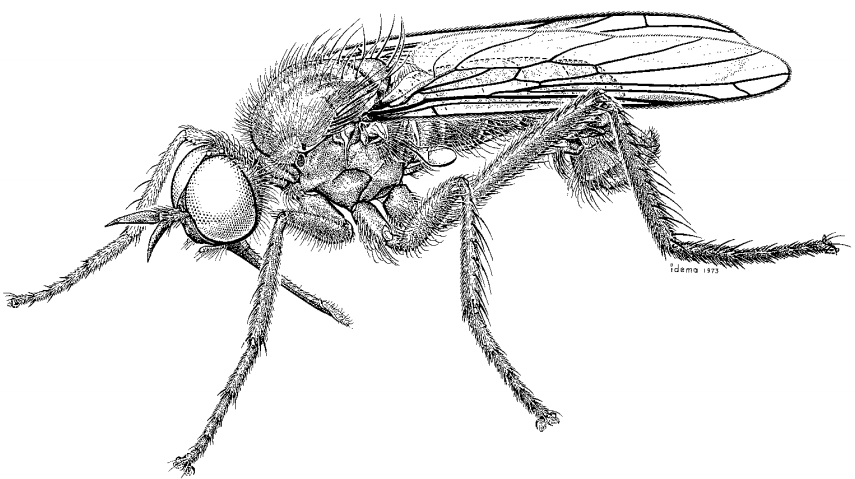
\includegraphics[width=\textwidth]{EmpididHabitus}
        \caption{Habitus \citep[][Fig. 47.1]{mcalpine1981manual}}
        \label{fig:empidid2}
    \end{subfigure}
    \caption{Empididae}\label{fig:empidids}
\end{figure}

\paragraph{Cyclorrhapha} The remaining flies are classified in Cyclorrhapha, a taxon that includes all flies that have a circular operculum on their puparia, through which they escape during eclosion.

\subsubsection{Pipunculidae (big-headed flies)}
\begin{itemize}
\item CuA2 reaches wing margin or joins A1 near margin
\item R4+5 do not branch, C ends at wing apex
\item antennae aristate
\item head strongly hemispherical, eyes LARGE
\item usually small, black and shiny
\end{itemize}

\noindent{}\textit{Natural history:} \\

\begin{figure}[ht!]
    \centering
    \begin{subfigure}[ht!]{0.45\textwidth}
        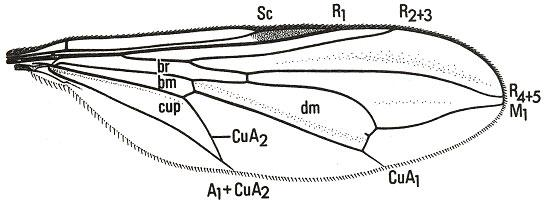
\includegraphics[width=\textwidth]{PipunculidWing}
        \caption{Fore wing \citep[][Fig. 4.50]{mcalpine1981manual}}
        \label{fig:pipunculid1}
    \end{subfigure}
    \qquad
    \begin{subfigure}[ht!]{0.42\textwidth}
        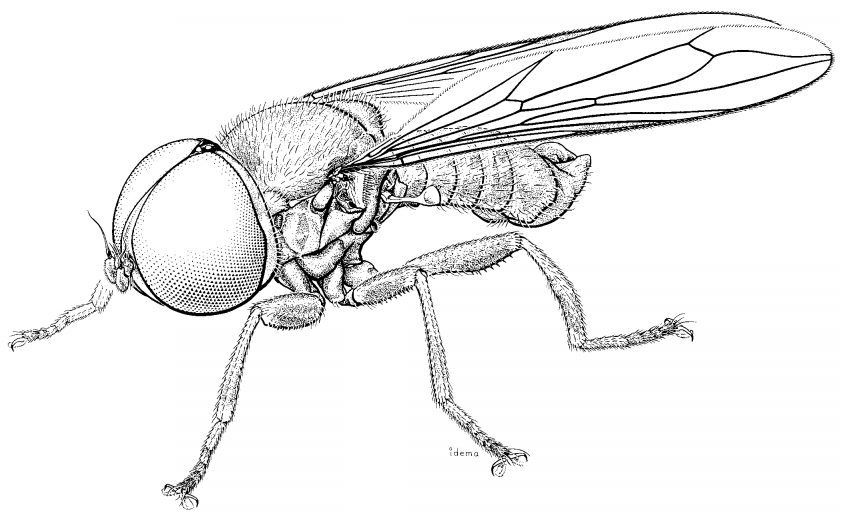
\includegraphics[width=\textwidth]{PipunculidHabitus}
        \caption{Habitus \citep[][Fig. 53.1]{mcalpine1981manualv2}}
        \label{fig:pipunculid2}
    \end{subfigure}
    \caption{Pipunculidae}\label{fig:pipunculids}
\end{figure}

\subsubsection{Syrphidae (hover, drone flies)}
\begin{itemize}
\item CuA2 reaches wing margin or joins A1 near margin
\item spurious vein present in wing between R and M
\item M1 usually curves up to meet R4+5  
\item antennae variable, often aristate
\item many mimic wasps and bees
\end{itemize}

\noindent{}\textit{Natural history:} \\

\begin{figure}[ht!]
    \centering
    \begin{subfigure}[ht!]{0.45\textwidth}
        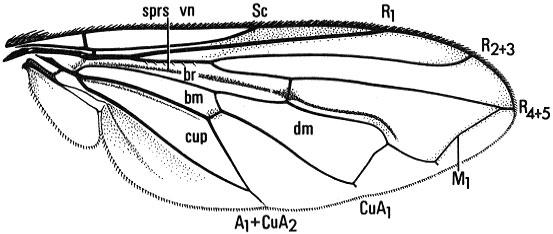
\includegraphics[width=\textwidth]{SyrphidWing}
        \caption{Fore wing \citep[][Fig. 52.52]{mcalpine1981manualv2}}
        \label{fig:syrphid2}
    \end{subfigure}
    \qquad 
    \begin{subfigure}[ht!]{0.45\textwidth}
        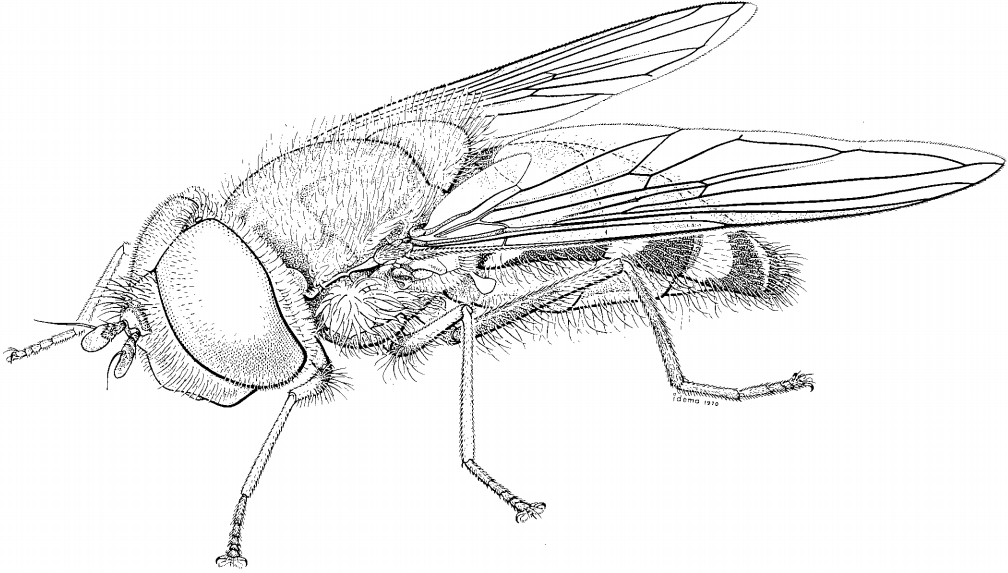
\includegraphics[width=\textwidth]{SyrphidHabitus}
        \caption{Habitus \citep[][Fig. 52.1]{mcalpine1981manualv2}}
        \label{fig:syrpidh1}
    \end{subfigure}
    \caption{Syrphidae}\label{fig:syrphids}
\end{figure}

\subsubsection{Phoridae (scuttle, coffin flies, \textit{etc}.)}
\begin{itemize}
\item CuA2 joins A1 far from margin
\item wings very distinct; Rs crowded anteriorly, 4--5 weak veins posteriorly
\item antennae flagellum globular with long arista
\item hind femora flattened
\item body somewhat humpbacked
\end{itemize}

\noindent{}\textit{Natural history:} \\

\begin{figure}[ht!]
    \centering
    \begin{subfigure}[ht!]{0.45\textwidth}
        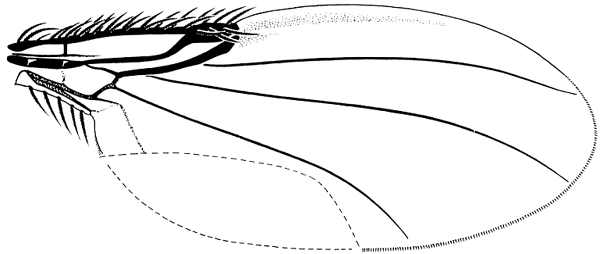
\includegraphics[width=\textwidth]{PhoridWing}
        \caption{Fore wing \citep[][Fig. 51.44]{mcalpine1981manualv2}}
        \label{fig:phorid1}
    \end{subfigure}
    \qquad
    \begin{subfigure}[ht!]{0.45\textwidth}
        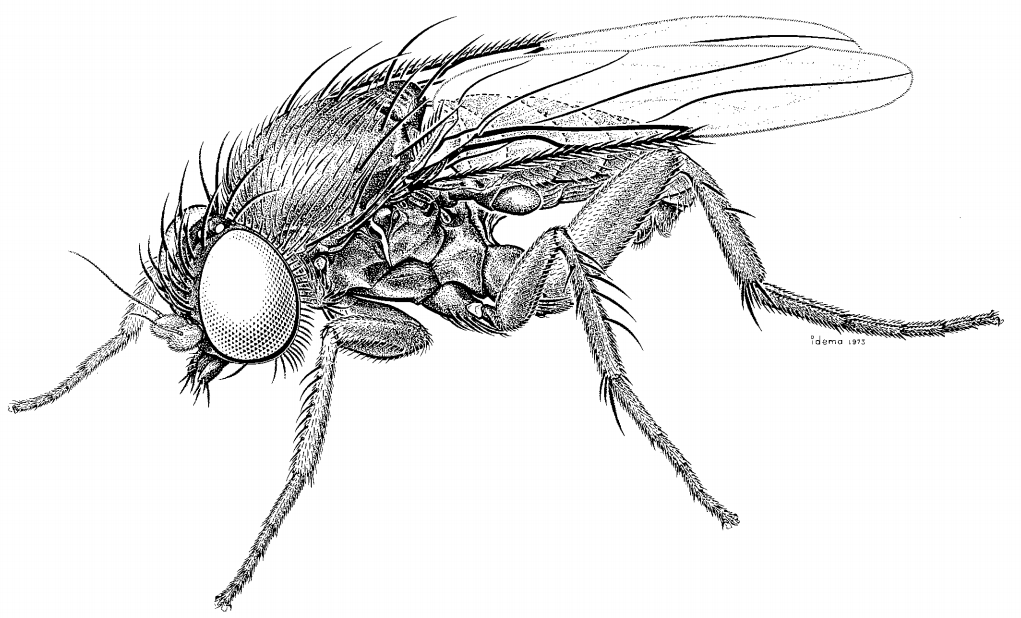
\includegraphics[width=\textwidth]{PhoridHabitus}
        \caption{Habitus \citep[][Fig. 51.1]{mcalpine1981manualv2}}
        \label{fig:phorid2}
    \end{subfigure}
    \caption{Phoridae}\label{fig:phorids}
\end{figure}

\paragraph{Schizophora} This taxon is thought to be monophyletic. It is comprised of species that usually share the following characteristics: 
\begin{itemize}
\item ptilinal suture (= frontal suture) present above the antennae; corresponds to structure (ptilinum) used to break out of puparium
\item CuA2 joins A1 far from margin
\item antennae almost always aristate
\end{itemize}
This taxon has traditionally been divided into two taxa, Acalyptratae and Calyptratae, based, in part, on the morphology of the fore wing. See below.

\paragraph{``Acalyptratae''} The next several families are commonly referred to as ``acalypterate flies'', a notoriously difficult group of flies to diagnose at almost any level. They generally share these character states:
\begin{itemize}
\item calypter almost always small to absent
\item transverse suture on thorax almost always absent
\item greater ampulla usually absent (bump near wing base, anterior to calypters)
\item antennal pedicel usually without complete dorsal seam
\item generally smaller and less setose than calyptrates
\item costa entire or broken; subcosta complete or incomplete (Figure \ref{fig:acalypteratewing})
\end{itemize}

\begin{figure}[ht!]
  \centering
    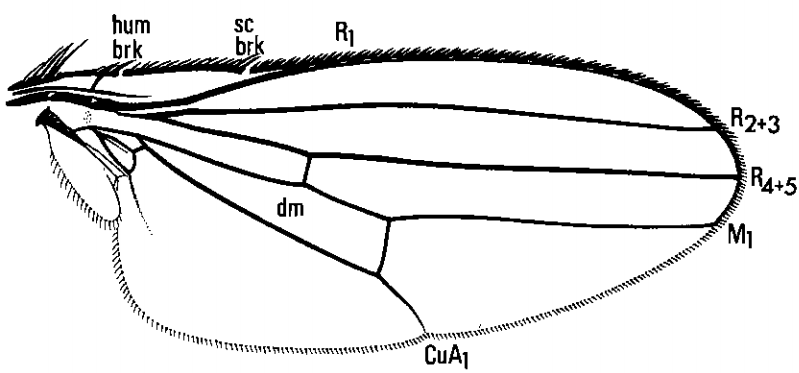
\includegraphics[width=0.5\textwidth]{AcalyptrateWing}
  \caption{Reference acalypterate wing \citep[][Fig. 4.59]{mcalpine1981manual}}
  \label{fig:acalypteratewing}
\end{figure}

%delete this one?
\subsubsection{Conopidae (thick-headed flies)}
\begin{itemize}
\item proboscis long, slender, usually 2× head
\item frontal suture sometimes apparently absent
\item antennae sometimes not aristate
\item M1 usually joins R4+5 so that there is an extra closed cell, sometimes crossvein between Sc and R
\item generally lacking large setae; many mimic wasps, atypical acalyptrates
\end{itemize}

\noindent{}\textit{Natural history:} \\

\begin{figure}[ht!]
    \centering
    \begin{subfigure}[ht!]{0.45\textwidth}
        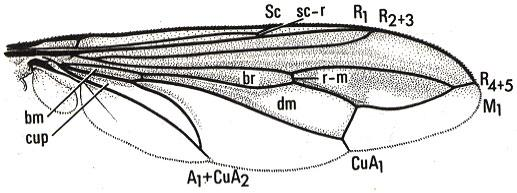
\includegraphics[width=\textwidth]{ConopidWing}
        \caption{Fore wing \citep[][Fig. 4.53]{mcalpine1981manual}}
        \label{fig:conopid1}
    \end{subfigure}
    \qquad
    \begin{subfigure}[ht!]{0.45\textwidth}
        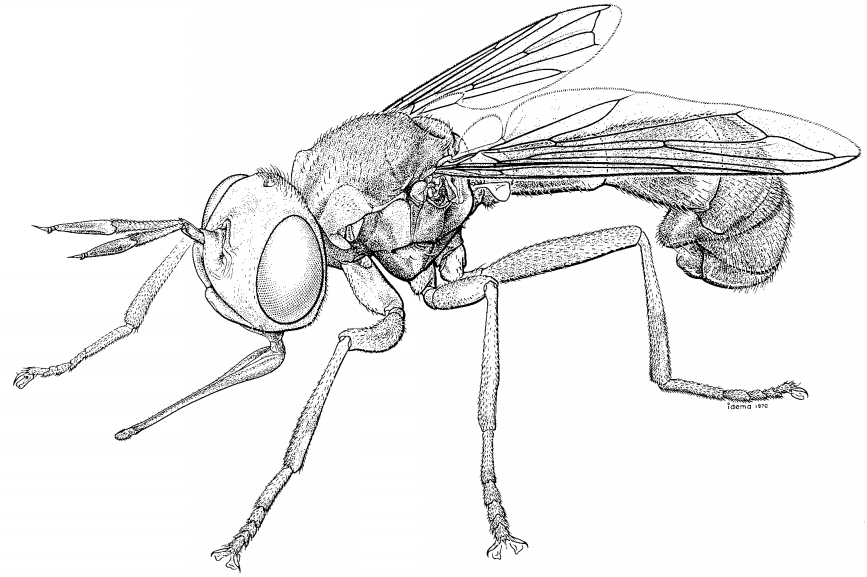
\includegraphics[width=\textwidth]{ConopidHabitus}
        \caption{Habitus \citep[][Fig. 54.1]{mcalpine1981manualv2}}
        \label{fig:conopid2}
    \end{subfigure}
    \caption{Conopidae}\label{fig:conopids}
\end{figure}

\subsubsection{Ulidiidae (picture-winged flies)}
\begin{itemize}
\item Sc complete, C usually entire
\item anal cell (cup in Figure \ref{fig:ulidiid1}) usually with acute projection posteriorly
\item apex of Sc not bending abruptly
\item oral vibrissae lacking (Figure \ref{fig:ulidiid2})
\item small to medium-sized, wings usually patterned
\end{itemize}

\noindent{}\textit{Natural history:} \\

\begin{figure}[ht!]
    \centering
    \begin{subfigure}[ht!]{0.47\textwidth}
        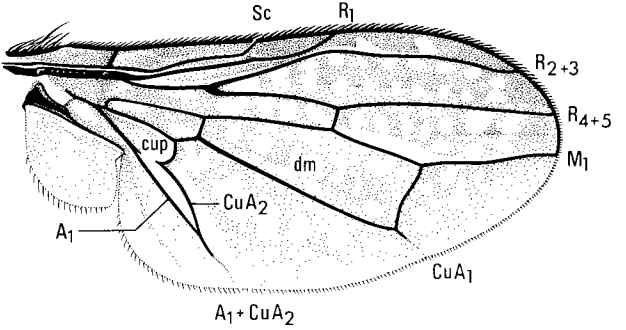
\includegraphics[width=\textwidth]{UlidiidWing}
        \caption{Fore wing \citep[][Fig. 63.15]{mcalpine1981manualv2}}
        \label{fig:ulidiid1}
    \end{subfigure}
    \qquad
    \begin{subfigure}[ht!]{0.26\textwidth}
        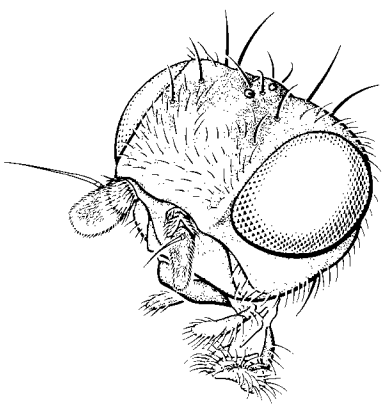
\includegraphics[width=\textwidth]{UlidiidHead}
        \caption{Head \citep[][Fig. 63.7]{mcalpine1981manualv2}}
        \label{fig:ulidiid2}
    \end{subfigure}
    \caption{Ulidiidae}\label{fig:ulidiids}
\end{figure}

\subsubsection{Tephritidae (fruit flies)}
\begin{itemize}
\item Sc usually incomplete, C usually broken
\item apex of Sc bent abruptly at end 
\item small to medium-sized, often patterned on wings, sometimes also on body
\item anal cell sometimes with acute projection (as in Ulidiidae)
\end{itemize}

\noindent{}\textit{Natural history:} \\

\begin{figure}[ht!]
    \centering
    \begin{subfigure}[ht!]{0.45\textwidth}
        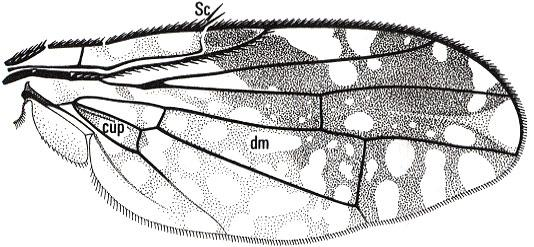
\includegraphics[width=\textwidth]{TephritidWing}
        \caption{Fore wing \citep[][Fig. 4.56]{mcalpine1981manual}}
        \label{fig:tephritid1}
    \end{subfigure}
    \qquad
    \begin{subfigure}[ht!]{0.4\textwidth}
        \includegraphics[width=\textwidth]{TephritidHabitus}
        \caption{Habitus \citep[][Fig. 66.1]{mcalpine1981manualv2}}
        \label{fig:tephritid2}
    \end{subfigure}
    \caption{Tephritidae}\label{fig:tephritids}
\end{figure}

\subsubsection{Agromyzidae (leafminer flies)}
\begin{itemize}
\item Sc incomplete, costa broken once
\item anal cell present
\item oral vibrissae present
\item postvertical bristles diverging
\item small, usually black and/or yellow, bristly
\end{itemize}

\noindent{}\textit{Natural history:} \\

\begin{figure}[ht!]
    \centering
    \begin{subfigure}[ht!]{0.45\textwidth}
        \includegraphics[width=\textwidth]{AgromyzidWing}
        \caption{Fore wing \citep[][Fig. 73.9]{mcalpine1981manualv2}}
        \label{fig:agromyzid1}
    \end{subfigure}
    \qquad
    \begin{subfigure}[ht!]{0.3\textwidth}
        \includegraphics[width=\textwidth]{AgromyzidHead}
        \caption{Head \citep[][Fig. 73.2]{mcalpine1981manualv2}}
        \label{fig:agromyzid2}
    \end{subfigure}
    \caption{Agromyzidae}\label{fig:agromyzids}
\end{figure}

\subsubsection{Chloropidae (grass or frit flies)}
\begin{itemize}
\item Sc incomplete, Costa broken once
\item anal cell absent
\item ocellar triangle greatly enlarged, usually shiny
\item oral vibrissae absent
\item diverse head shapes, smooth, very few setae
\item tiny, often colorful flies
\end{itemize}

\noindent{}\textit{Natural history:} \\

\begin{figure}[ht!]
    \centering
    \begin{subfigure}[ht!]{0.5\textwidth}
        \includegraphics[width=\textwidth]{ChloropidWing}
        \caption{Fore wing \citep[][Fig. 99.36]{mcalpine1981manualv2}}
        \label{fig:chloropid1}
    \end{subfigure}
    \qquad
    \begin{subfigure}[ht!]{0.25\textwidth}
        \includegraphics[width=\textwidth]{ChloropidHead}
        \caption{Head \citep[][Fig. 99.3]{mcalpine1981manualv2}}
        \label{fig:chloropid2}
    \end{subfigure}
    \caption{Chloropidae}\label{fig:chloropids}
\end{figure}

\subsubsection{Drosophilidae (pomace, vinegar flies)}
\begin{itemize}
\item Sc incomplete, costa broken twice
\item anal cell present
\item postvertical bristles converging
\item arista plumose
\item oral vibrissae present
\item usually small, yellowish, brownish, or grayish
\end{itemize}

\noindent{}\textit{Natural history:} \\

\begin{figure}[ht!]
    \centering
    \begin{subfigure}[ht!]{0.5\textwidth}
        \includegraphics[width=\textwidth]{DrosophilidWing}
        \caption{Fore wing \citep[][Fig. 95.6]{mcalpine1981manualv2}}
        \label{fig:drosophilid1}
    \end{subfigure}
    \qquad
    \begin{subfigure}[ht!]{0.27\textwidth}
        \includegraphics[width=\textwidth]{DrosophilidHead}
        \caption{Head \citep[][Fig. 95.6]{mcalpine1981manualv2}}
        \label{fig:drosophilid2}
    \end{subfigure}
    \caption{Drosophilidae}\label{fig:drosophilids}
\end{figure}
%%%%%%%%%%%%%%%%%%%%%%%%%%%% here!
\paragraph{Calyptratae} The remaining families are part of an apparently monophyletic taxon called Calyptratae, named for the expanded calypters of the fore wing. These insects also usually have the following characters:
\begin{itemize}
\item transverse suture complete on thorax
\item greater ampulla (bump at base of wing, anterior to calypters) present, enlarged 
\item antennal pedicel with complete dorsal seam
\item generally larger, more setose than acalyptrates
\end{itemize}

\begin{figure}[ht!]
  \centering
    \includegraphics[width=0.8\textwidth]{CalyptrateMorph}
  \caption{Calyptratae morphology; \textbf{ar} = arista, \textbf{mr} = meron, \textbf{npl} = notopleuron, \textbf{npl s} = notopleural seta, \textbf{sbsctl} = subscutellum, \textbf{sctl} = scutellum \citep[][Fig. 2.66]{mcalpine1981manual}}
  \label{fig:calyptratemorph}
\end{figure}

\subsubsection{Muscidae (house flies and relatives)}
\begin{itemize}
\item usually drab but is also variable in color and form
\item meron without row of bristles
\item no setae present on ventral surface of scutellum
\item fore wing \texorpdfstring{A\textsubscript{1}}{A1} short and not reaching margin
\item \texorpdfstring{R\textsubscript{5}}{R5} cell parallel-sided or narrowing distally
\end{itemize}

\noindent{}\textit{Natural history:} \\

\begin{figure}[ht!]
    \centering
    \begin{subfigure}[ht!]{0.4\textwidth}
        \includegraphics[width=\textwidth]{MuscidWings}
        \caption{Fore wings \citep[][Fig. 105.22,24]{mcalpine1981manualv2}}
        \label{fig:muscid1}
    \end{subfigure}
    \qquad
    \begin{subfigure}[ht!]{0.45\textwidth}
        \includegraphics[width=\textwidth]{MuscidHabitus}
        \caption{Habitus \citep[][Fig. 105.1]{mcalpine1981manualv2}}
        \label{fig:muscid2}
    \end{subfigure}
    \caption{Muscidae}\label{fig:muscids}
\end{figure}

\subsubsection{Anthomyiidae (anthomyiid flies)}
\begin{itemize}
\item meron without row of bristles
\item \texorpdfstring{A\textsubscript{1}}{A1} reaching wing margin, at least as fold
\item \texorpdfstring{R\textsubscript{5}}{R5} cell always parallel-sided
\item scutellum with setae ventrally 
\item hairs often present under scutellum
\item almost always drab: black, gray, brown
\item thinner abdomen and lighter color than Muscidae
\end{itemize}

\noindent{}\textit{Natural history:} \\

\begin{figure}[ht!]
    \centering
    \begin{subfigure}[ht!]{0.5\textwidth}
        \includegraphics[width=\textwidth]{AnthomyiidWing}
        \caption{Fore wing \citep[][Fig. 104.29]{mcalpine1981manualv2}}
        \label{fig:anthomyiid1}
    \end{subfigure}
    \qquad
    \begin{subfigure}[ht!]{0.4\textwidth}
        \includegraphics[width=\textwidth]{AnthomyiidThorax}
        \caption{Thorax \citep[][Fig. 104.18]{mcalpine1981manualv2}}
        \label{fig:anthomyiid2}
    \end{subfigure}
    \caption{Anthomyiidae}\label{fig:anthomyiids}
\end{figure}

\subsubsection{Tachinidae (parasitic flies)}
\begin{itemize}
\item subscutellum developed (sbsctl in Figure \ref{fig:calyptratemorph})
\item \texorpdfstring{R\textsubscript{5}}{R5} cell narrowed or closed distally
\item arista usually not plumose (Figure \ref{fig:tachinid1})
\item meron with row of bristles (see Figure \ref{fig:calyptratemorph}, near hind coxa (cx 3))
\end{itemize}

\noindent{}\textit{Natural history:} \\

\begin{figure}[ht!]
    \centering
    \begin{subfigure}[ht!]{0.5\textwidth}
        \includegraphics[width=\textwidth]{TachinidWing}
        \caption{Fore wing \citep[][Fig. 110.201]{mcalpine1981manualv2}}
        \label{fig:tachinid1}
    \end{subfigure}
    \qquad
    \begin{subfigure}[ht!]{0.21\textwidth}
        \includegraphics[width=\textwidth]{TachinidHead}
        \caption{Head in lateral view \citep[][Fig. 110.91]{mcalpine1981manualv2}}
        \label{fig:tachinid2}
    \end{subfigure}
    \caption{Tachinidae}\label{fig:tachinids}
\end{figure}

\subsubsection{Calliphoridae (blow flies)}
\begin{itemize}
\item often (but not always!) metallic in color
\item arista plumose
\item meron with row of bristles
\item 2 notopleural bristles present
\item \texorpdfstring{R\textsubscript{5}}{R5} cell narrowed or closed distally
\end{itemize}

\noindent{}\textit{Natural history:} \\

\begin{figure}[ht!]
    \centering
    \begin{subfigure}[ht!]{0.5\textwidth}
        \includegraphics[width=\textwidth]{CalliphoridWing}
        \caption{Fore wing \citep[][Fig. 106.6]{mcalpine1981manualv2}}
        \label{fig:calliphorid1}
    \end{subfigure}
    \qquad
    \begin{subfigure}[ht!]{0.3\textwidth}
        \includegraphics[width=\textwidth]{CalliphoridHead}
        \caption{Head in dorsal view \citep[][Fig. 106.18]{mcalpine1981manualv2}}
        \label{fig:calliphorid2}
    \end{subfigure}
    \caption{Calliphoridae}\label{fig:calliphorids}
\end{figure}

\subsubsection{Sarcophagidae (flesh flies)}
\begin{itemize}
\item not metallic, generally thorax with black/gray stripes, apex of abdomen usually reddish or orange
\item arista usually plumose only on proximal half (Figure \ref{fig:sarcoph2})
\item meron with row of bristles
\item usually 4 notopleural bristles present, rarely 3
\item \texorpdfstring{R\textsubscript{5}}{R5} cell narrowed or closed distally
\end{itemize}

\noindent{}\textit{Natural history:} \\

\begin{figure}[ht!]
    \centering
    \begin{subfigure}[ht!]{0.5\textwidth}
        \includegraphics[width=\textwidth]{SarcophagidWing}
        \caption{Fore wing \citep[][Fig. 116.30]{mcalpine1981manualv2}}
        \label{fig:sarcoph1}
    \end{subfigure}
    \qquad
    \begin{subfigure}[ht!]{0.25\textwidth}
        \includegraphics[width=\textwidth]{SarcophagidHead}
        \caption{Head in antero-lateral view \citep[][Fig. 116.13]{mcalpine1981manualv2}}
        \label{fig:sarcoph2}
    \end{subfigure}
    \caption{Sarcophagidae}\label{fig:sarcophs}
\end{figure}

\subsubsection{Hippoboscidae (louse flies)}
\begin{itemize}
\item highly modified, louse-like in shape, often wingless 
\item body setae relatively short
\item eyes often very small
\item coxae widely separated
\item venation reduced, Rs located anteriorad of typical position in Diptera
\item wings sometimes dehiscent (wings fell off of specimen)
\item segmentation on abdomen indistinct
\end{itemize}

\noindent{}\textit{Natural history:} \\

\begin{figure}[ht!]
    \centering
    \begin{subfigure}[ht!]{0.45\textwidth}
        \includegraphics[width=\textwidth]{HippoboscidHabitus}
        \caption{Winged female \citep[][Fig. 111.1]{mcalpine1981manualv2}}
        \label{fig:hippoboscid1}
    \end{subfigure}
    \qquad
    \begin{subfigure}[ht!]{0.35\textwidth}
        \includegraphics[width=\textwidth]{HippoboscidFemale}
        \caption{Wingless female \citep[][Fig. 111.36]{mcalpine1981manualv2}}
        \label{fig:hippoboscid2}
    \end{subfigure}
    \caption{Hippoboscidae}\label{fig:hippoboscids}
\end{figure}

\FloatBarrier

\section*{Acknowledgments}
Andrew R. Deans and Istv\'an Mik\'o wrote the text. Most of the illustrations were generously made available by Agriculture Canada. Our reproduction of the illustrations from this work is not produced in affiliation with, or with the endorsement of the Government of Canada.

\FloatBarrier
% adding bibliography here
\bibliographystyle{apalike}
\bibliography{bib}

\end{document}
